\subsection{Derivative Trade Lifecycle}
\label{sec:derivative_trade_lifecycle}

The derivative trade lifecycle refers to the process that a derivatives contract goes through from its initiation to its final settlement (Figure \ref{fig:trade-lifecycle}). This lifecycle consists of several stages, each critical to the completion of the trade \citep{isda_market_infrastructure}.

\begin{itemize}
    \item \textbf{Trade Initiation}. The lifecycle of a derivative trade begins with the initiation of a contract. This involves the agreement on various aspects such as the type of derivative being traded (e.g., futures, options, swaps), the underlying asset on which the derivative is based, the size of the contract, the price, and the expiry date of the contract. This stage is crucial as it establishes the primary terms and conditions that will govern the trade.

    \begin{itemize}
        \item \textbf{Payment of Upfront Premium}. In some derivatives like options, an upfront premium is often required. This is a payment made at the beginning of the contract to secure the rights provided by the derivative. The premium is usually non-refundable and paid by the option buyer to the option seller. The payment of this premium is crucial as it can affect the profitability and risk profile of the trade. Failure to pay the premium may result in the cancellation of the contract.
    \end{itemize}

    \item \textbf{Trade Execution}. After the contract terms are decided upon, the trade is executed. The execution creates a legal obligation between the parties involved. This means they are now legally bound to uphold their end of the agreement. This can occur on an exchange, where standardized contracts are traded, or over-the-counter (OTC), where contracts can be customized to fit the needs of the parties involved.

    \item \textbf{Trade Confirmation}. Following execution, trade confirmation takes place. This involves the communication between the trading parties to verify the terms of the deal. The aim is to ensure that both parties agree on the details and understand their obligations. This process minimizes the risk of a trade failing due to miscommunication or misunderstanding.
    
    \item \textbf{Trade Clearing}. After trade confirmation, clearing occurs. A clearinghouse or a central counterparty (CCP) becomes involved at this stage. The CCP stands between the buyer and seller, essentially becoming the buyer to every seller and the seller to every buyer. This reduces counterparty risk — the risk that one party may default on its contractual obligations. The clearinghouse also handles the administration of the trade, from validation of the transaction to maintaining records.

    \item \textbf{Trade Settlement and Reporting}. Upon reaching its expiration date, the derivative contract is settled. The exact nature of the settlement depends on the type of derivative and the terms of the contract. It could involve a cash settlement or the physical delivery of the underlying asset. The process concludes with the reporting of the transaction for record-keeping and regulatory purposes. Any profit or loss is realized at this stage.

    \begin{itemize}
        \item \textbf{Multiple Payments Over Time}. For derivatives like interest rate swaps or certain types of structured products, there may be multiple payments that occur over a potentially very long time, sometimes spanning years. These payments are usually outlined in the initial contract and are subject to variables like interest rates or asset performance. The timing and amount of these payments are critical elements in the risk and return profile of the derivative.
    \end{itemize}

    \item \textbf{Post-Trade Events}. After the trade is settled and reported, any post-trade events are handled. This might include the monitoring and management of any remaining risk, the calculation and payment of taxes, and any necessary compliance reporting.
\end{itemize}

Each stage of the trade lifecycle involves a variety of market participants, including the original trading parties, brokers, exchanges, clearinghouses, and regulatory bodies. Each of these actors plays a crucial role in ensuring that the trade is completed efficiently, transparently, and in compliance with all applicable rules and regulations.

\begin{figure}[!h]
    \centering
    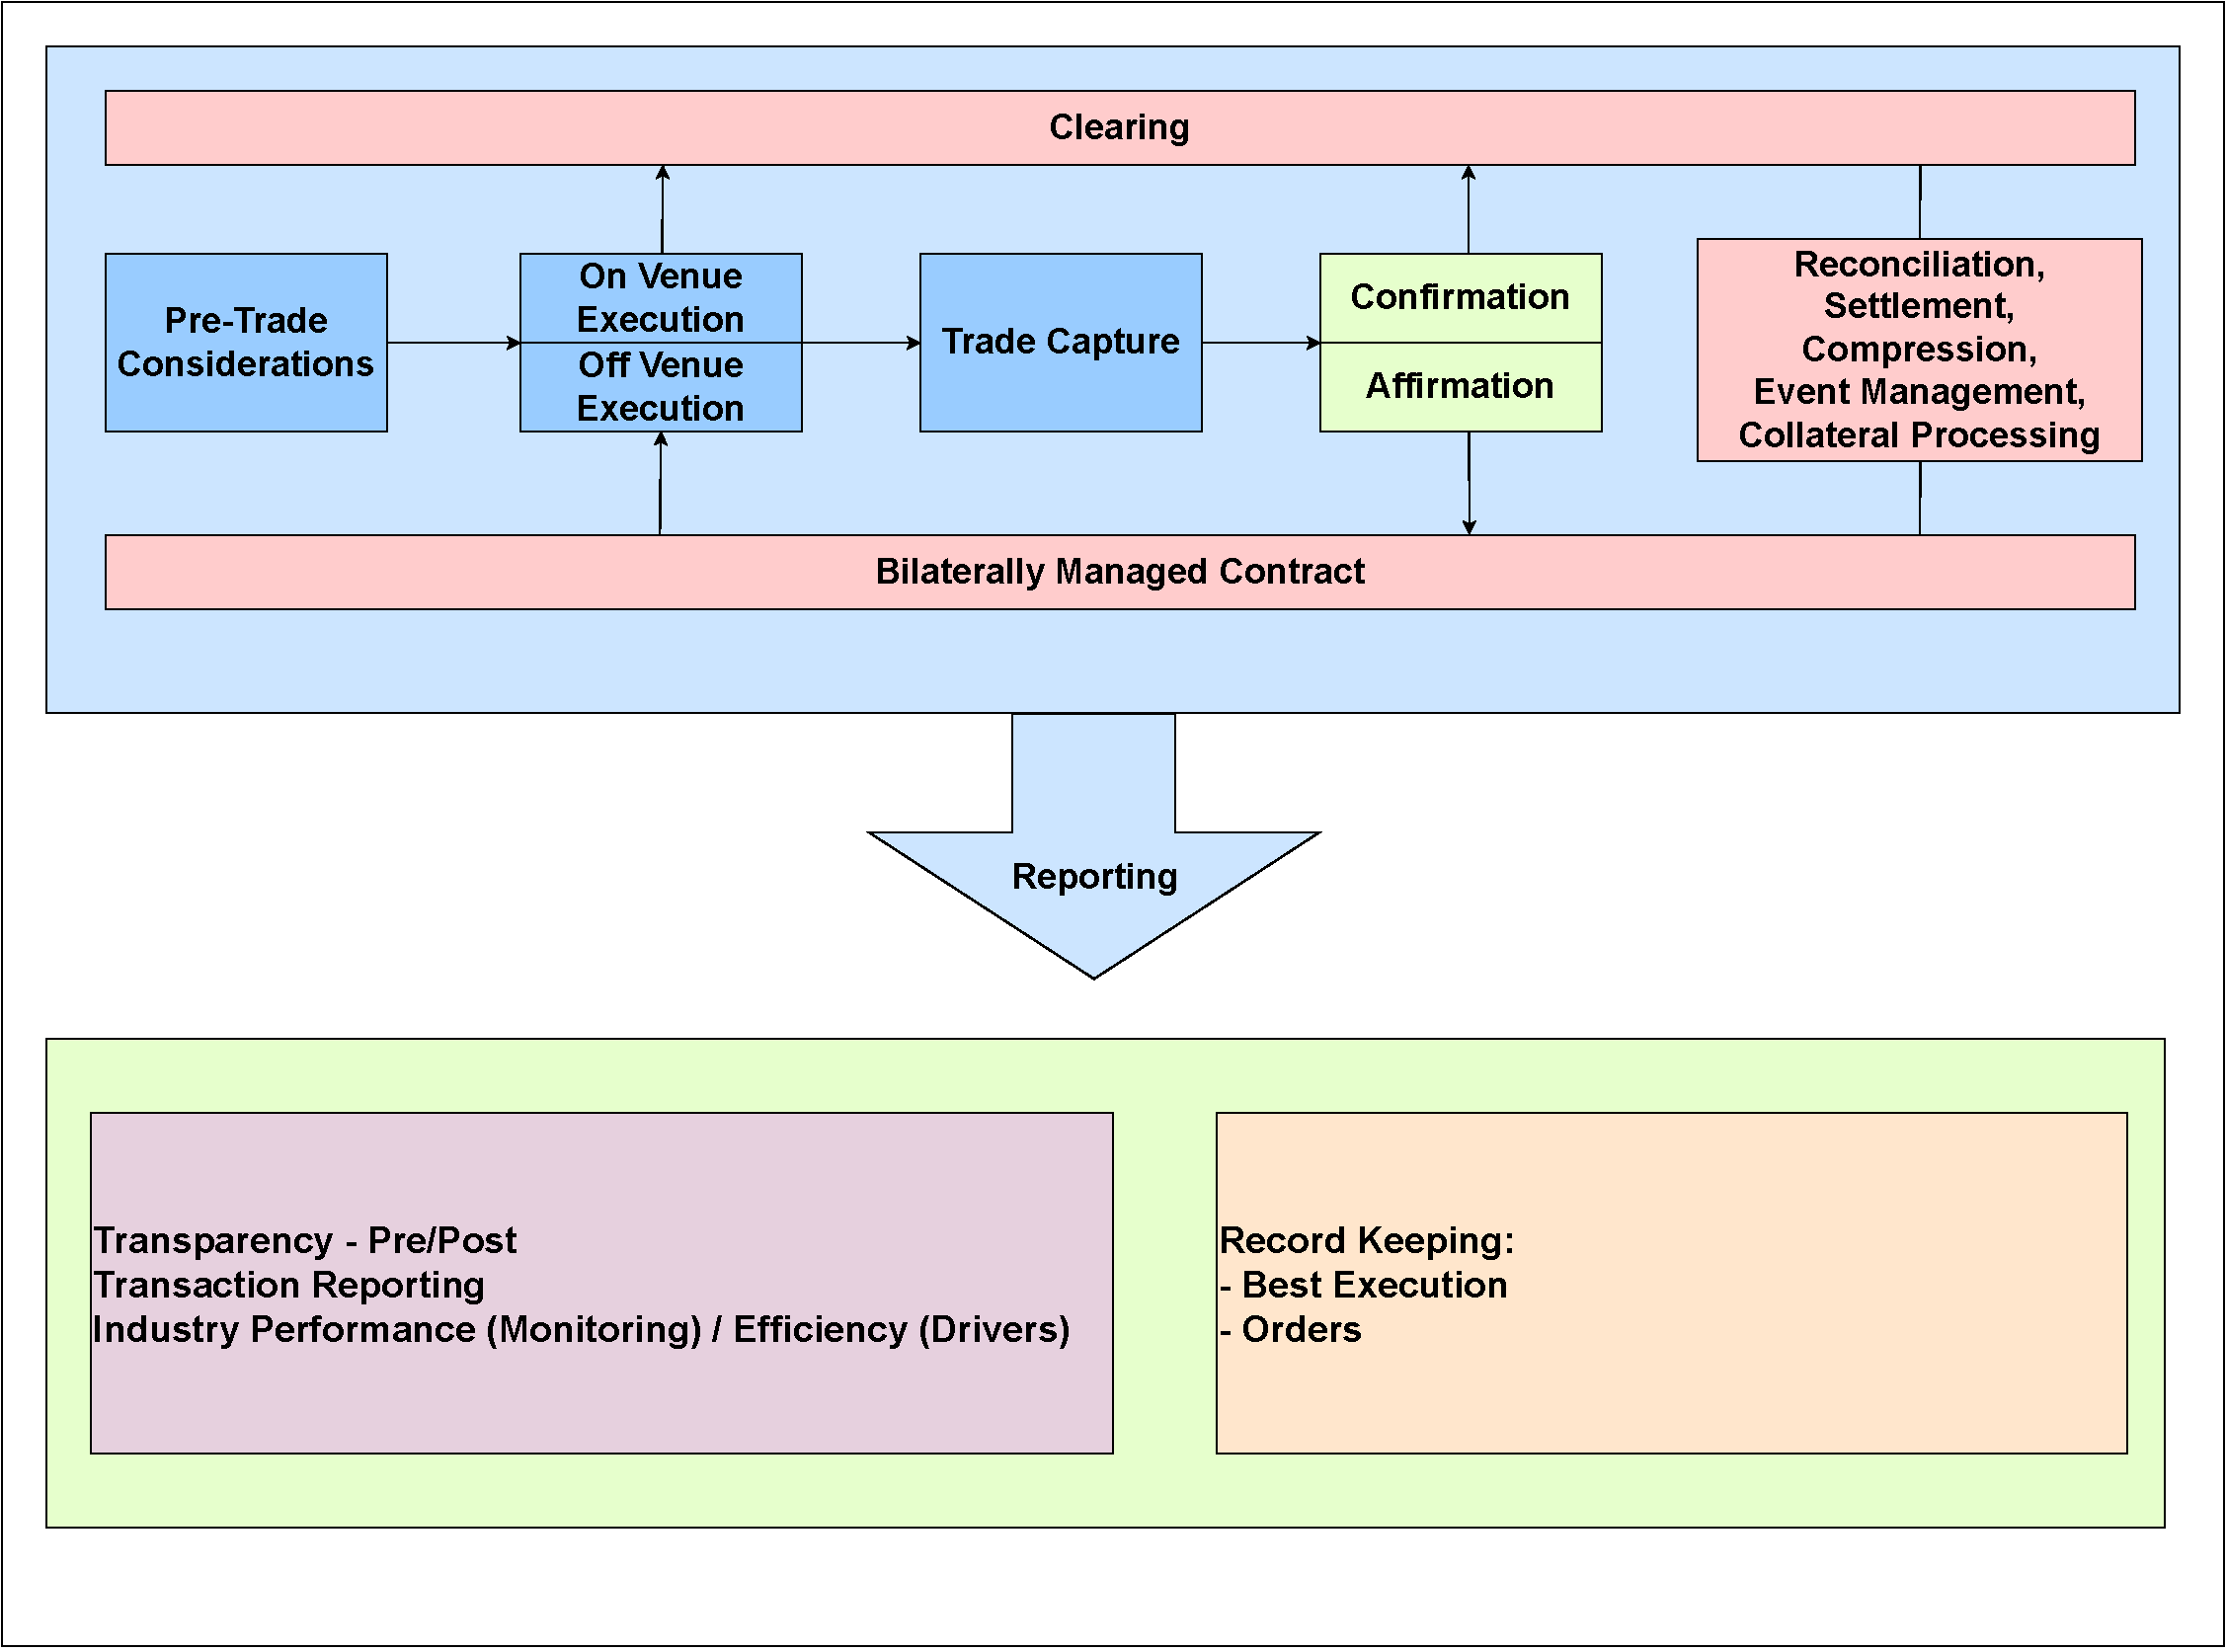
\includegraphics[width=\textwidth]{images/chapter-2/trade-lifecycle.pdf}
    \caption[Derivative Trade Lifecycle]{Adapted from \citep{isda_market_infrastructure}. The steps involved in the lifecycle of a derivative trade as per ISDA definition \citep{isda_market_infrastructure}. Starting with \textit{pre-trade considerations}, parties assess market conditions, risks, and regulatory implications to align their trading strategies. The \textit{trade execution} can either be on-venue, on regulated platforms, or off-venue, directly between parties. Once executed, the trade's details are meticulously captured, followed by a thorough \textit{confirmation and affirmation} process to ensure accuracy and mutual agreement. This leads into a multifaceted phase of \textit{portfolio reconciliation,} \textit{settlement}, \textit{compression} (reducing the number of derivative contracts in a portfolio without altering its net risk profile), \textit{event management}, and \textit{collateral processing}, ensuring both parties have matching records, finalizing the trade, managing lifecycle events, and mitigating credit risks. The \textit{clearing} stage introduces a central counterparty, guaranteeing trade terms and reducing default risks. Comprehensive §\textit{reporting} to authorities ensures transparency and compliance, while diligent \textit{record-keeping} tracks trade history and adherence to best execution practices.
    
    }
    \label{fig:trade-lifecycle}
\end{figure}